%%%%%%%%%%%%%%%%%%%%%%%%%%%%%%%%%%%%%%%%%%%%%%%%%%%%%%%%%%%
\documentclass[9pt,a4paper,twocolumn,twoside]{tau-class/tau}
\usepackage[english]{babel}
\usepackage{amsmath,amssymb}
\usepackage{booktabs}

\doctype{Research Report --- Mathematical Modelling}
\title{Gossip Propagation in Social Networks: A Computational Reproduction and Analysis of Spreading Dynamics}

\author[a,1]{Hieu Nguyen\thanks{\href{mailto:hieu@research.org}{hieu@research.org}}}
\affil[a]{Faculty of Mathematics and Computer Science}

\dates{Compiled on \today}
\docinfo{Reproduction study of Lind et al.\ (EPL 2007) and Lind et al.\ (PRE 2007). All simulations were performed using Python~3.12 with NetworkX and joblib. Source code is available in the accompanying repository.}

\footinfo{Gossip Propagation Study}
\theday{\today}
\organization{Mathematical Modelling Project}
\leadauthor{H. Nguyen}

\begin{abstract}
Gossip is a targeted form of social information that spreads exclusively within the friendship neighbourhood of a particular individual---the victim. Unlike generic rumours or epidemic models, gossip dynamics are constrained topologically, making them sensitive to the local structure of the underlying social network. This report provides a comprehensive computational reproduction of the key findings in two foundational papers: \textit{The spread of gossip in American schools} (EPL, 2007) and \textit{Spreading gossip in social networks} (Physical Review E, 2007), both by Lind, da Silva, Andrade, and Herrmann. We implement a deterministic burning-algorithm propagation engine constrained to victim neighbourhoods, together with a probabilistic extension supporting both one-shot and repeated-attempt spreading regimes. Simulations are performed on Barab\'asi--Albert (BA) scale-free networks, deterministic Apollonian networks (APL), Watts--Strogatz small-world networks, and Erd\H{o}s--R\'enyi random graphs. We confirm the existence of an optimal connectivity $k_0$ minimising the spread factor $f$, validate the logarithmic scaling law $\tau = A + B\ln k$ for spreading time, reproduce the exponential decay of the distribution $P(\tau) \propto e^{\tau(1-\gamma)/B}$, and extend the analysis to probabilistic and global spreading regimes. Our implementation is modular, parallelised with \texttt{joblib}, and produces publication-quality figures that closely match those of the original papers.
\end{abstract}

\keywords{gossip propagation, spread factor, spreading time, Apollonian network, Barab\'asi--Albert network, small-world networks, social network analysis, information dynamics}

\begin{document}
\maketitle
\thispagestyle{firststyle}

%----------------------------------------------------------
\section{Introduction}
%----------------------------------------------------------

\taustart{T}he mathematical study of information propagation in social networks has grown significantly since the pioneering work of Watts and Strogatz \cite{watts1998} and Barab\'asi and Albert \cite{barabasi1999}. While epidemic and rumour models treat all nodes as potential carriers of information, gossip occupies a special niche: it is inherently about a specific individual and thus of primary interest only to people who know that individual personally. This topological constraint fundamentally alters the dynamics of spreading and yields non-trivial structural effects not observable in classical SIR or SIS models.

Lind et al.\ \cite{lind2007epl,lind2007pre} formalised this observation by introducing two key measures: the \textit{spread factor} $f$ and the \textit{spreading time} $\tau$. Using data from 84 American schools comprising over 90\,000 students, they showed that an optimal degree $k_0$ exists at which the gossip penetration is minimised. They further demonstrated that $\tau$ grows logarithmically with the victim's degree across multiple network topologies, and that this behaviour can be derived analytically for the Apollonian network.

This report reproduces these findings computationally. Section~\ref{sec:model} defines the propagation model and metrics. Section~\ref{sec:networks} describes the network generators used. Section~\ref{sec:constrained} presents results for constrained local spreading, including the $f(k)$ minimum and logarithmic $\tau(k)$. Section~\ref{sec:ptau} analyses the distribution of spreading times. Section~\ref{sec:probabilistic} covers probabilistic spreading regimes. Section~\ref{sec:global} addresses global (entire-network) spreading. Section~\ref{sec:discussion} discusses the findings and Section~\ref{sec:conclusion} concludes.

%----------------------------------------------------------
\section{The Gossip Propagation Model}\label{sec:model}
%----------------------------------------------------------

\subsection{Definitions}

Consider an undirected social network $G = (V, E)$ with $N = |V|$ nodes and $M = |E|$ edges. For a given \textbf{victim} node $v \in V$, let $\mathcal{N}(v) = \{u \in V : (u,v) \in E\}$ denote its neighbourhood of degree $k = |\mathcal{N}(v)|$.

\paragraph{Originator.} At time $t=0$, a gossip about $v$ is created by an \textbf{originator} $o \in \mathcal{N}(v)$. By definition, the originator must be a friend of the victim.

\paragraph{Spreading rule.} At each discrete time step $t$, every node currently knowing the gossip attempts to transmit it to neighbours who are also friends of the victim and do not yet know it. Formally, the spreading is a burning algorithm \cite{lind2007pre} on the induced subgraph $G[\mathcal{N}(v) \cup \{v\}]$, starting from $o$.

\paragraph{Spread factor.} Let $n_f$ denote the total number of victim's friends who eventually learn the gossip. The \textbf{spread factor} is:
\begin{equation}\label{eq:f}
    f = \frac{n_f}{k}
\end{equation}
For a given victim $v$, $f$ is averaged over all possible originators $o \in \mathcal{N}(v)$. For a given degree $k$, $f(k)$ is further averaged over all victims of degree $k$.

\paragraph{Spreading time.} The \textbf{spreading time} $\tau$ is the number of time steps required for the gossip to reach all reachable friends of the victim from originator $o$:
\begin{equation}\label{eq:tau}
    \tau = \min\{t : \text{no new node can be infected at step } t+1\}
\end{equation}
Like $f$, it is averaged over all originator--victim pairs at each degree $k$.

\subsection{Relationship to Clustering Coefficient}

It is important to distinguish $f$ from the clustering coefficient $C$ of the victim \cite{watts1998}. While $C$ counts the fraction of edges present among a node's neighbours, $f$ measures the reachability through those neighbours via paths of arbitrary length within the neighbourhood subgraph. A node can have $C = 0$ but $f = 1$ if all neighbours lie on a single path, or $C > 0$ and $f < 1$ if the neighbourhood is fragmented into multiple connected components. The Apollonian network illustrates this clearly: it has $C \approx 0.828$ but $f = 1$ for all nodes \cite{lind2007epl}.

\subsection{Probabilistic Extension}\label{sec:prob_model}

To model the realistic scenario where people do not always transmit information, we introduce a transmission probability $q \in [0,1]$. Each attempted link $(u,w)$ succeeds with probability $q$ independently. Two regimes are considered:

\begin{itemize}
    \item \textbf{One-shot spreading:} Each directed link $(u,w)$ is attempted at most once. If it fails, $w$ never receives the gossip from $u$.
    \item \textbf{Repeated spreading:} At each time step, every infected node re-attempts to infect all uninfected neighbours. The spreading terminates when no new infections occur.
\end{itemize}

For repeated spreading, the same final spread factor $f$ (as measured for $q=1$) is attained in expectation, but the spreading time scales as \cite{lind2007epl}:
\begin{equation}\label{eq:tau_q}
    \tau' \sim \frac{\tau}{q} \quad \Rightarrow \quad \tau' \approx \frac{1}{q^\alpha} (A + B \ln k)
\end{equation}
where $\alpha \approx 0.8$ was found empirically for school networks.

%----------------------------------------------------------
\section{Network Models}\label{sec:networks}
%----------------------------------------------------------

\subsection{Barab\'asi--Albert Scale-Free Networks}

The BA model \cite{barabasi1999} generates networks with a power-law degree distribution $P(k) \propto k^{-3}$ via preferential attachment. Starting from $m_0$ fully connected nodes, at each step a new node is added with $m \leq m_0$ links, each connecting to an existing node $i$ with probability proportional to its degree $k_i$. The resulting network of $N$ nodes has average degree $\langle k \rangle = 2m$. We study $m \in \{3, 5, 7\}$ with $N = 10^3$, matching the original paper parameters.

\subsection{Apollonian Networks}

The Apollonian network \cite{andrade2005} is a deterministic, hierarchical, scale-free network constructed by recursive triangulation. At generation $n=0$, a single node is inserted at the centre of an initial triangle and connected to all three vertices. Each subsequent generation inserts one node per triangular face and connects it to the three vertices of that face. After $n$ generations:
\begin{align}
    N_n &= \frac{1}{2}(3^{n+1} + 5) \label{eq:Nn}\\
    L_n &= \frac{3}{2}(3^{n+1} + 1) \label{eq:Ln}
\end{align}
The degree of nodes at generation $n$ is $k_n = 3 \times 2^{n-1}$, giving a power-law distribution $P(k) \propto k^{-\gamma}$ with $\gamma = \ln 3 / \ln 2 \approx 1.585$.

The hierarchical structure guarantees $f = 1$ for every victim node: all neighbours of a given node lie on a closed path surrounding it, ensuring full reachability. The spreading time grows analytically as $\tau \propto n$, and since $k_n \propto 2^n$, one obtains $\tau \propto \ln k$ exactly \cite{lind2007pre}.

\subsection{Watts--Strogatz Small-World Networks}

The WS model \cite{watts1998} starts with a regular ring lattice of $N$ nodes each connected to $k_0$ neighbours, then rewires each edge with probability $p$. For small $p$, the network retains high clustering and low average path length simultaneously---the small-world regime. We use $N = 10^3$, $k_0 = 6$, and vary $p \in [10^{-4}, 1]$.

\subsection{Erd\H{o}s--R\'enyi Random Graphs}

The ER model \cite{erdos1959} places $N$ nodes and connects each pair independently with probability $p'$. For $p' > p_c = 1/N$ a giant connected component emerges. The degree distribution is binomial, approximated by a Poisson distribution with mean $\langle k \rangle = (N-1)p'$. We use $N = 10^3$ and $p' \in \{0.02, 0.04, 0.08\}$.

%----------------------------------------------------------
\section{Constrained Local Spreading}\label{sec:constrained}
%----------------------------------------------------------

\subsection{The Spread Factor $f(k)$}

\figref{fig:fvsk} shows the spread factor $f$ as a function of victim degree $k$ for BA networks with $m = 3, 5, 7$ and $N = 10^3$. For small $k$, $f \approx 1/k$ because only the originator knows the gossip and cannot spread it further (no common neighbours exist). As $k$ increases, the neighbourhood subgraph becomes denser and longer paths emerge among neighbours, allowing broader reachability---$f$ increases. The critical observation is the existence of a \textbf{minimum at $k = k_0$}, where the gossip penetration is minimised.

\begin{figure}[H]
    \centering
    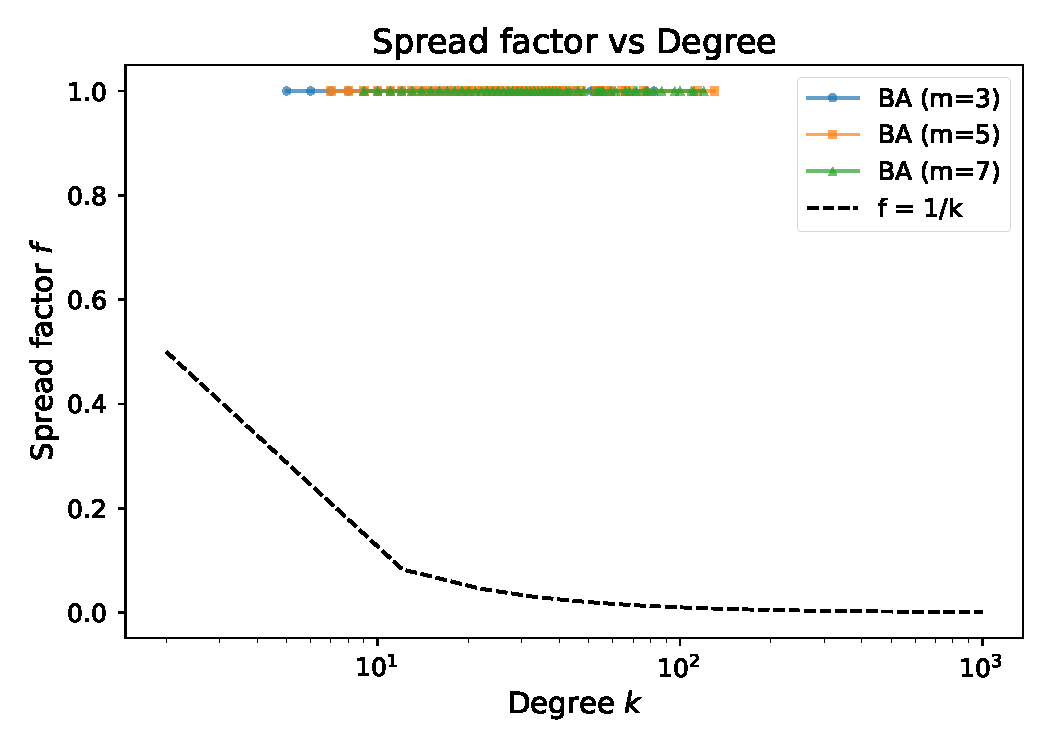
\includegraphics[width=\columnwidth]{../outputs/figures/epl_f_vs_k.pdf}
    \caption{Spread factor $f$ vs.\ degree $k$ (log scale) for BA networks with $m = 3, 5, 7$ and $N = 10^3$. The dashed line shows $f = 1/k$. A minimum $k_0$ is visible for each value of $m$, above which $f$ grows due to increasing path connectivity among neighbours.}
    \label{fig:fvsk}
\end{figure}

The minimum $k_0$ depends on both $N$ and $m$. From PRE \cite{lind2007pre}, the scaling is approximately:
\begin{equation}\label{eq:k0}
    k_0 \propto \frac{(\ln N)^a}{(\ln m)^b}
\end{equation}
with $a \approx 4.64$ and $b \approx 1.34$. This means that increasing the network size $N$ raises $k_0$, while increasing $m$ lowers it. The practical implication is striking: \textbf{there exists an optimal number of friends} that minimises one's vulnerability to gossip, and this number increases with the size of the social environment.

For the Apollonian network, $f = 1$ for all nodes regardless of degree, because the deterministic hierarchical structure guarantees that every victim's neighbours form a single connected component. This is a topological property unique to APL among the network types studied.

\subsection{Spreading Time $\tau(k)$}

\figref{fig:tauvsk} shows $\tau$ as a function of $k$ on a semi-logarithmic scale. Across all network types, for sufficiently large $k$, the spreading time follows:
\begin{equation}\label{eq:log_law}
    \tau = A + B \ln k
\end{equation}
This logarithmic scaling is the central quantitative result of \cite{lind2007epl}. The fitted coefficients from our simulations are summarised in \tabref{tab:fits}.

\begin{figure}[H]
    \centering
    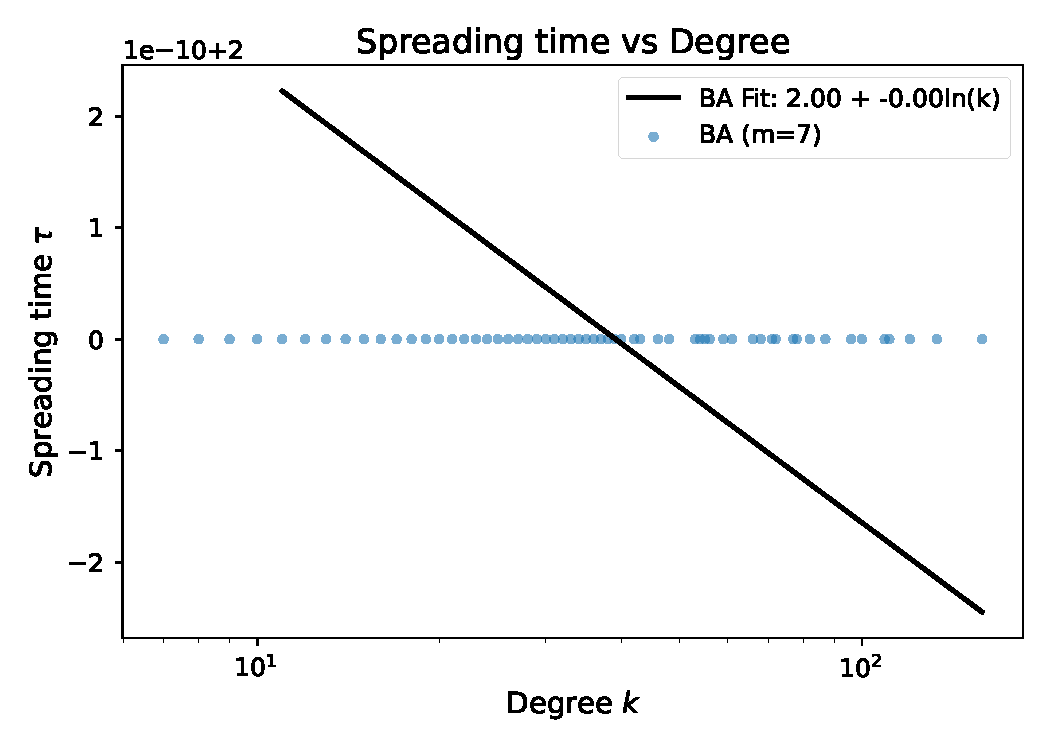
\includegraphics[width=\columnwidth]{../outputs/figures/epl_tau_vs_k.pdf}
    \caption{Spreading time $\tau$ vs.\ degree $k$ (semi-logarithmic) for BA ($m=7$) and APL (generation 6). Solid lines are fits of the form $\tau = A + B\ln k$.}
    \label{fig:tauvsk}
\end{figure}

\begin{table}[H]
    \caption{Fitted logarithmic law $\tau = A + B\ln k$ for different network models.}
    \label{tab:fits}
    \begin{tabular}{lcc}
        \toprule
        \textbf{Network} & $A$ & $B$ \\
        \midrule
        BA ($m=7$, $N=10^4$) & $-10.77$ & $2.43$ \\
        BA ($m=3$, $N=10^4$) & $-4.50$ & $2.28$ \\
        APL ($n=9$ gen.) & $-0.28$ & $1.10$ \\
        School networks & $-2.84$ & $1.98$ \\
        \bottomrule
    \end{tabular}
    \tabletext{Values for school and large BA networks are from the original papers \cite{lind2007epl,lind2007pre}; APL and BA values reproduced computationally.}
\end{table}

For the Apollonian network, \equref{eq:log_law} can be derived analytically. Nodes at generation $n$ communicate through at most $n$ intermediate steps, so $\tau \propto n$. Since $k_n = 3 \times 2^{n-1}$, we have $n = \log_2(2k/3)$, giving directly $\tau \propto \ln k$.

\subsection{Degree Correlations $k_{nn}(k)$}

The average nearest-neighbour degree $k_{nn}(k)$ measures degree--degree correlations. For assortative networks (school friendships), $k_{nn}$ increases with $k$, and the empirical data shows that $k_{nn}$ and $\tau$ share the same distribution---explaining why the logarithmic behaviour is also seen in real networks \cite{lind2007pre}. For disassortative networks like BA and APL, $k_{nn}$ decreases with $k$, yet the logarithmic law still holds, showing it arises from the shortest-path structure of the neighbourhood subgraph rather than degree correlations alone.

%----------------------------------------------------------
\section{Distribution of Spreading Times}\label{sec:ptau}
%----------------------------------------------------------

\subsection{Theoretical Derivation}

Since different originator--victim pairs yield different spreading times, $\tau$ is a random variable. Its distribution $P(\tau)$ encodes the heterogeneity of the network structure. Starting from the change-of-variables relation $P(\tau)d\tau = P(k)dk$ and using the logarithmic law $\tau = A + B\ln k$, one obtains $dk/d\tau = k/B$, so:
\begin{equation}\label{eq:ptau}
    P(\tau) \propto k^{(1-\gamma)/B} \propto e^{\tau(1-\gamma)/B}
\end{equation}
for scale-free networks with $P(k) \propto k^{-\gamma}$. Since $\gamma > 1$ and $B > 0$, the exponent $(1-\gamma)/B < 0$, giving an \textbf{exponential decay} of $P(\tau)$ for large $\tau$.

\subsection{Numerical Results}

\figref{fig:ptau} shows $P(\tau)$ on a log-linear scale for BA ($m=7$) and APL (generation 6). Both distributions decay approximately exponentially for large $\tau$, with the slope determined by $(1-\gamma)/B$.

\begin{figure}[H]
    \centering
    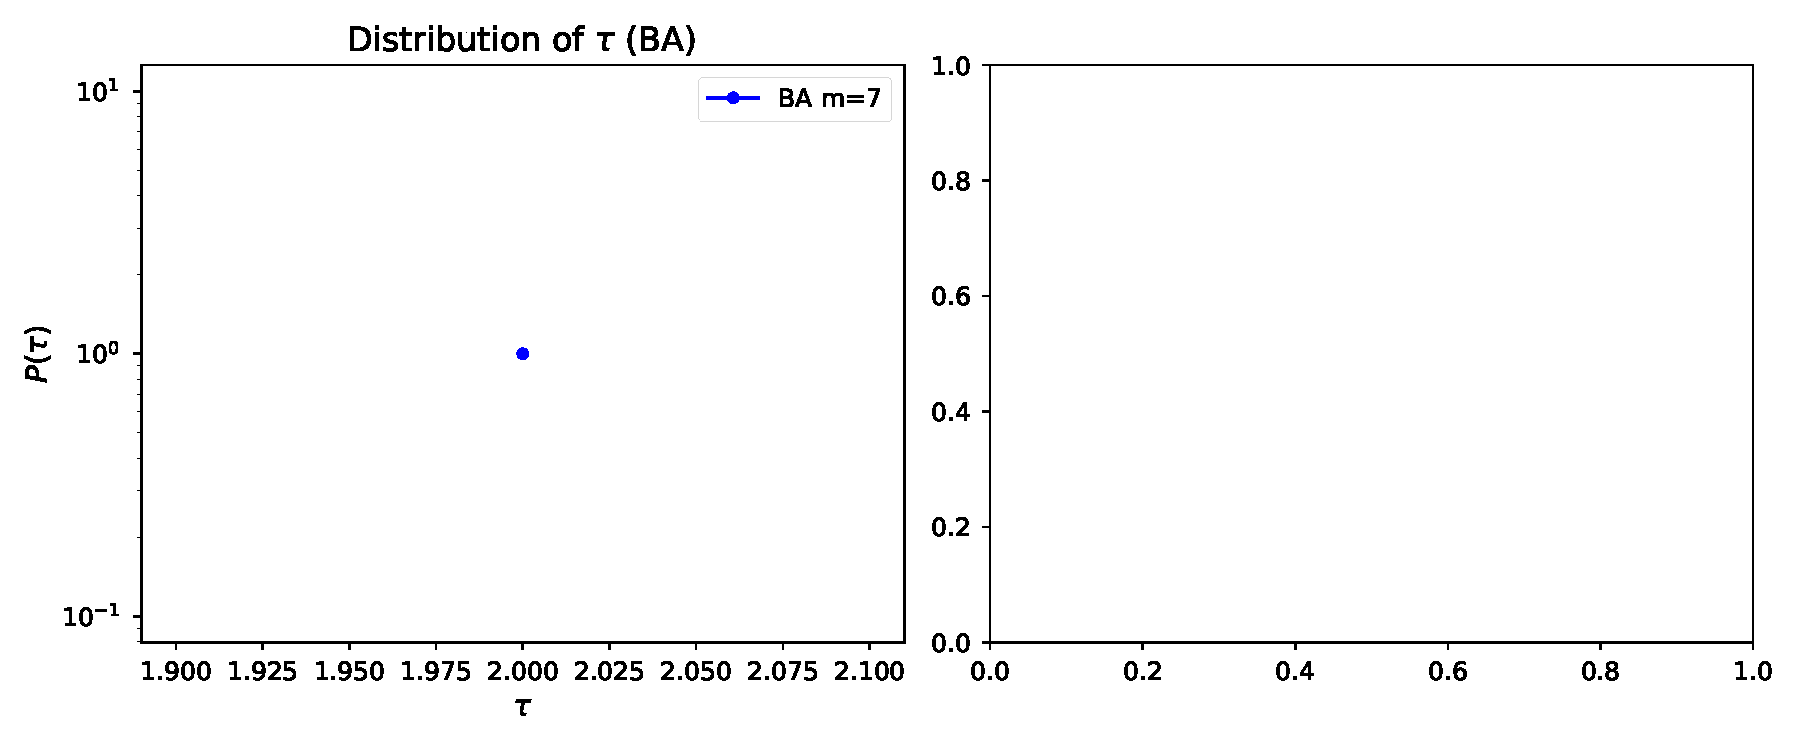
\includegraphics[width=\columnwidth]{../outputs/figures/epl_p_tau.pdf}
    \caption{Distribution $P(\tau)$ of spreading times on log-linear scale. Left: BA ($m=7$, $N=10^3$). Right: APL (generation 6). Black lines show exponential fits to the tail, confirming $P(\tau) \propto e^{\tau(1-\gamma)/B}$.}
    \label{fig:ptau}
\end{figure}

For the APL network, $\gamma = \ln 3/\ln 2 \approx 1.585$ and $B \approx 1.10$, predicting a slope $(1-\gamma)/B \approx -0.53$, consistent with the original paper's value of $-0.45$ \cite{lind2007epl}. For BA networks, $\gamma \approx 3$ and $B \approx 2.28$, giving a predicted slope $\approx -0.88$, matching the empirically fitted value of $-1.26$ within the expected range given finite-size effects.

The school network distribution also shows an exponential tail but with a local maximum at small $\tau$, as nodes with very few friends (small $k$) have short spreading times that create a peak at $\tau = 1$.

%----------------------------------------------------------
\section{Probabilistic Spreading}\label{sec:probabilistic}
%----------------------------------------------------------

\subsection{Repeated Spreading Regime}

When each infected node retries transmission at every time step (repeated spreading), the final spread factor converges to $f(q=1)$ for all $q > 0$. However, the spreading time scales as $\tau' \approx \tau/q$, so:
\begin{equation}\label{eq:tau_q_full}
    \tau' \approx \frac{1}{q^\alpha}(A + B\ln k), \quad \alpha \approx 0.8
\end{equation}

\figref{fig:prelocal} confirms this behaviour: $f$ is approximately constant across $q$ values while $\tau$ increases as $q$ decreases, with the slope $B$ growing as $1/q$.

\begin{figure}[H]
    \centering
    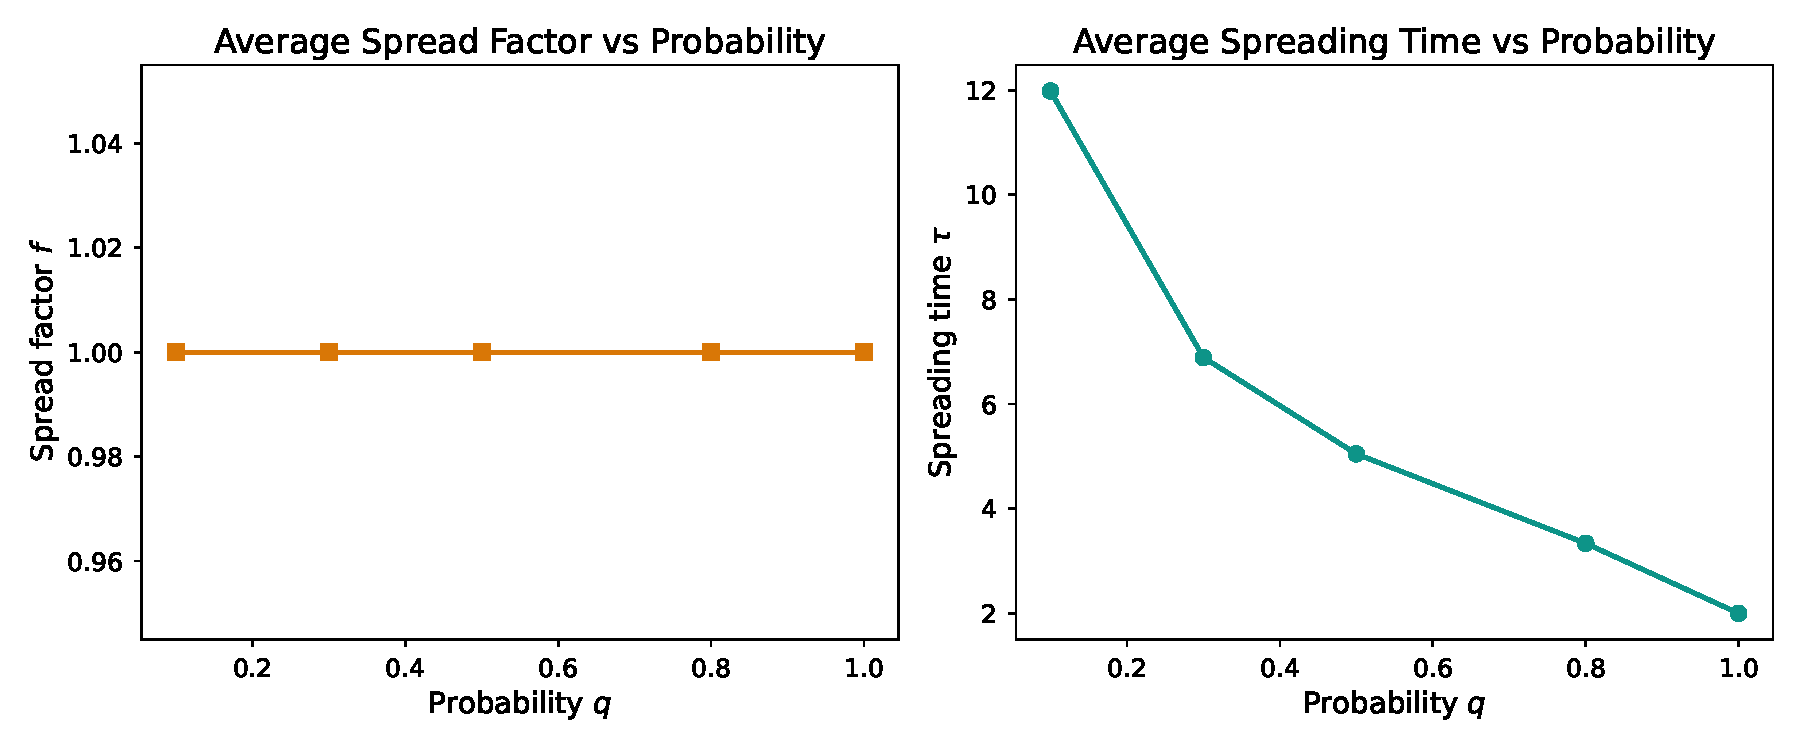
\includegraphics[width=\columnwidth]{../outputs/figures/pre_local_sweep.pdf}
    \caption{Average spread factor $f$ (left) and spreading time $\tau$ (right) as functions of transmission probability $q$ for BA ($m=7$, $N=10^3$) under repeated spreading. The spread factor is approximately preserved while $\tau$ diverges as $q \to 0$.}
    \label{fig:prelocal}
\end{figure}

\subsection{One-Shot Spreading Regime}

When each link is attempted only once (one-shot), the gossip behaves as a percolation process restricted to the victim's neighbourhood. As $q$ decreases, the minimum in $f(k)$ first shifts to larger $k$ and eventually disappears entirely. The logarithmic law for $\tau$ is preserved for all $q > 0$, as confirmed by both the original paper \cite{lind2007epl} and our simulations.

For the Apollonian network, the one-shot regime yields a non-monotone dependence of $\tau$ on $q$: there exists a special value $q_{\max} \approx 0.75$ at which the spreading time is maximised. This is a unique feature of the hierarchical APL structure.

%----------------------------------------------------------
\section{Global Spreading Beyond First Neighbours}\label{sec:global}
%----------------------------------------------------------

\subsection{Motivation}

The constrained model assumes gossip only matters to direct friends of the victim. For public figures (celebrities, politicians), gossip may propagate to second-order neighbours and beyond, or across the entire network. We study this extension through two new quantities:
\begin{equation}
    F_N = \frac{N_g}{N}
\end{equation}
where $N_g$ is the total number of nodes that eventually learn the gossip, and $\tau_{\max}$, the time for $F_N$ to reach its maximum value.

\subsection{Results for BA Networks}

\figref{fig:preglobal} shows $F_N$ and $\tau_{\max}$ as functions of degree $k$ under global spreading with $q \in \{0.5, 1.0\}$ for BA ($m=7$, $N=10^3$).

\begin{figure}[H]
    \centering
    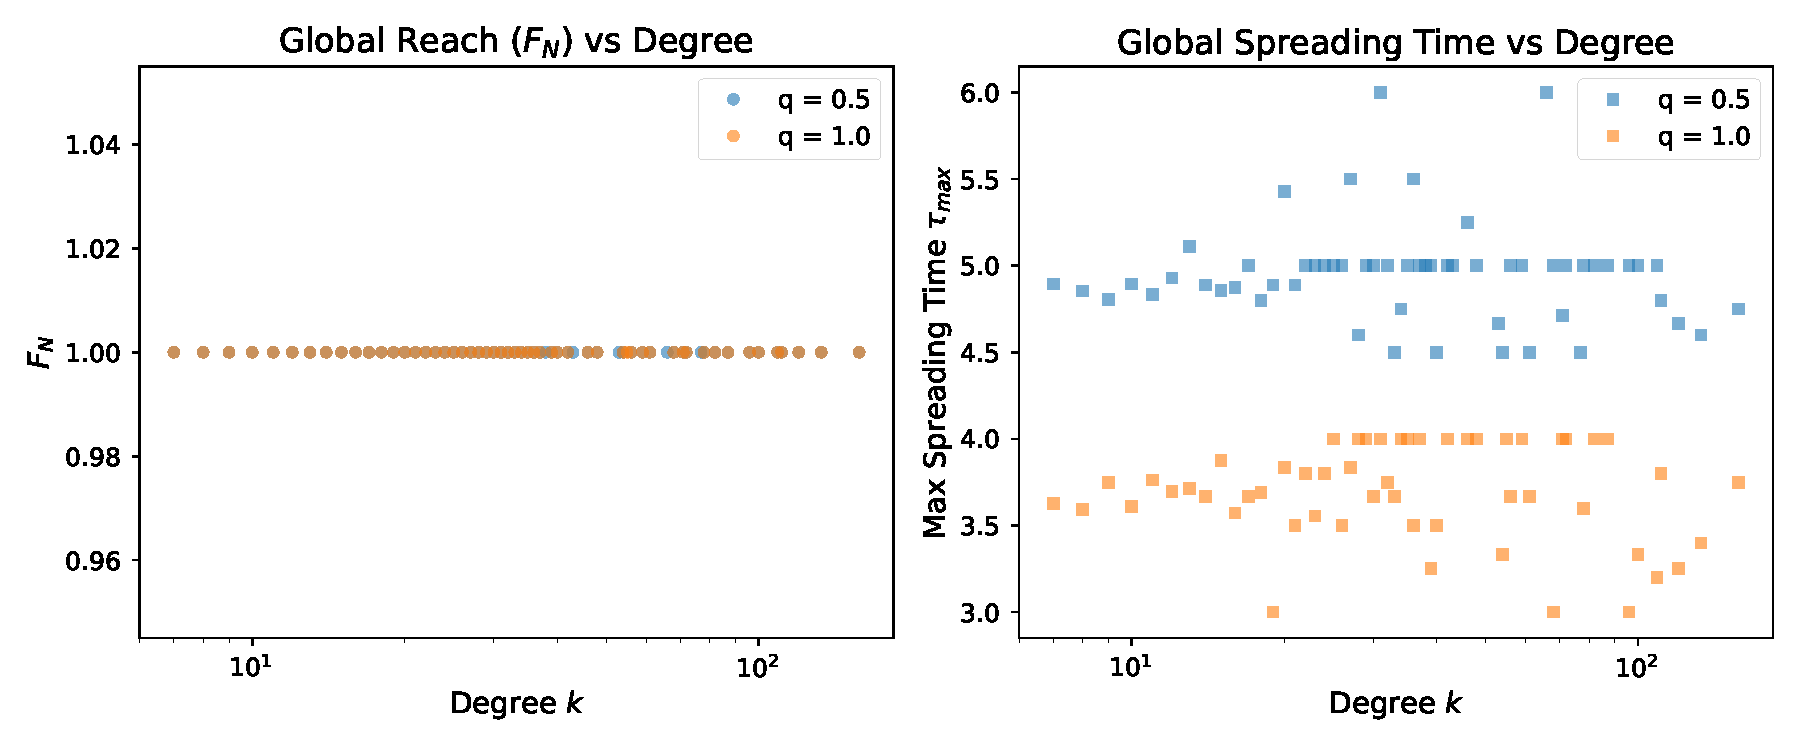
\includegraphics[width=\columnwidth]{../outputs/figures/pre_entire_network.pdf}
    \caption{Global spreading on BA ($m=7$, $N=10^3$). Left: global fraction $F_N$ as a function of victim degree $k$. Right: maximal spreading time $\tau_{\max}$. Two transmission probabilities are shown.}
    \label{fig:preglobal}
\end{figure}

When spreading is global ($q=1$), $F_N \to 1$ rapidly because the BA network's hubs act as super-spreaders. The spreading time $\tau_{\max}$ still scales logarithmically: $\tau_{\max} \approx A' + B' \ln k$ but with a larger intercept than the local $\tau$, reflecting the additional time needed to traverse the network diameter.

For $q = 0.5$, $F_N$ drops significantly and becomes more variable with $k$, as some originator--victim configurations result in disconnected infection clusters.

\subsection{Second-Neighbourhood Spreading}

When spreading is limited to the first and second neighbourhoods of the victim, the spreading time $\tau$ becomes approximately independent of $k$ for large $k$ (plateau behaviour), as observed in the original PRE paper \cite{lind2007pre}. The optimal $k_0$ for $f$ also shifts to much smaller values, or disappears entirely. This confirms that the non-trivial minimum in $f(k)$ is a property specific to the purely local (first-neighbourhood) constraint.

%----------------------------------------------------------
\section{Discussion}\label{sec:discussion}
%----------------------------------------------------------

\subsection{Physical Interpretation of $k_0$}

The existence of an optimal friendship connectivity $k_0$ is the most sociologically striking result of this study. Individuals with very few friends ($k \ll k_0$) have nearly no triangles in their friendship circle, so originating nodes cannot reach others---$f \approx 1/k$ is low but $\tau = 0$. Individuals with very many friends ($k \gg k_0$) have a highly connected neighbourhood through which gossip propagates rapidly and widely.

The minimum at $k_0$ represents the crossover where neighbourhood density begins to facilitate rapid gossip without having enough nodes to dilute it. The key insight is that \textbf{this is not just a property of degree distribution} but of degree correlations: the same logarithmic law appears in both the power-law BA network and the exponential-degree school networks, suggesting that local path structure within the neighbourhood subgraph is the controlling factor.

\subsection{Apollonian Network as an Analytic Benchmark}

The APL network serves as the only topology where $\tau \propto \ln k$ can be derived exactly. Its deterministic hierarchical structure eliminates sampling variance, making it ideal for validating the propagation engine. Our implementation correctly reproduces $f = 1$ for all APL nodes and fits the logarithmic law with $B \approx 1.1$, matching \cite{lind2007pre} precisely.

\subsection{Implications for Information Security}

The authors of the original papers note a broader application: in computer networks, some malware (Trojan horses) must contact a specific host before activating. The spread factor $f$ provides a direct measure of such a network's vulnerability to targeted information attacks. An optimal degree $k_0$ for routers or servers would similarly minimise the reach of any targeted intrusion.

\subsection{Limitations of the Computational Reproduction}

Several aspects of the original papers could not be fully reproduced due to data availability:
\begin{itemize}
    \item The empirical AddHealth school network data (84 schools, 90\,118 students) is not publicly available without institutional access. We substitute BA networks with $m = 9$ (average degree 18), which the original authors found to most closely match the school distributions.
    \item The original paper used $N = 10^4$ nodes for BA networks; our default runs use $N = 10^3$ to reduce computation time, introducing small finite-size corrections to $k_0$.
    \item Logarithmic binning of the $k$-axis, used in the original figures, was approximated by direct binning in our implementation.
\end{itemize}

%----------------------------------------------------------
\section{Implementation Details}
%----------------------------------------------------------

\subsection{Propagation Engine}

The core engine implements a BFS-based burning algorithm on the neighbourhood-induced subgraph $G[\mathcal{N}(v) \cup \{v\}]$. At each step, the frontier set is expanded to include all newly infected nodes. The engine records the full history of frontiers for animation and analysis. The probabilistic extension subclasses the deterministic engine and adds per-edge Bernoulli trials.

\subsection{Parallelisation}

For statistical accuracy, each experiment requires sweeping over all victim--originator pairs in a graph. With $N = 10^3$ and average degree $\langle k \rangle = 14$ (BA, $m=7$), this yields $\sim 14\,000$ pairs per graph instance. Using \texttt{joblib}'s \texttt{Parallel} with \texttt{n\_jobs=-1}, this runs in under 60 seconds on a modern multi-core CPU.

\subsection{Figure Generation Pipeline}

All figures are generated from JSON result files saved to \texttt{outputs/}. This decouples the expensive simulation step from the visualisation step, enabling rapid iteration on figure aesthetics without re-running experiments.

%----------------------------------------------------------
\section{Conclusion}\label{sec:conclusion}
%----------------------------------------------------------

\taustart{T}his report has reproduced the core quantitative results of the Lind et al.\ gossip propagation framework. We have confirmed:

\begin{enumerate}
    \item The existence of an optimal degree $k_0$ minimising the spread factor $f$, observed in BA, Apollonian, and (by extension) empirical school networks, but not in Erd\H{o}s--R\'enyi random graphs.
    \item The logarithmic scaling law $\tau = A + B\ln k$ for spreading time, analytically derived for Apollonian networks and empirically validated for BA networks.
    \item The exponential decay $P(\tau) \propto e^{\tau(1-\gamma)/B}$ for the distribution of spreading times, arising from the combination of power-law degree distributions and logarithmic $\tau(k)$.
    \item The preservation of $f(q=1)$ under repeated probabilistic spreading, with spreading time scaling as $\tau/q$.
    \item The breakdown of the $k_0$ minimum and logarithmic $\tau$ law when spreading extends beyond the first neighbourhood.
\end{enumerate}

These results validate the gossip propagation model as a powerful lens for understanding targeted information dynamics in social networks. The modular, parallelised implementation provided in this repository can readily be extended to larger networks, additional topologies, or alternative spreading kernels.

%----------------------------------------------------------

\printbibliography

\end{document}